\RequirePackage{amsmath}
\RequirePackage{fix-cm}
\documentclass[deutsch]{svmono}

\def\ColoredLinks{}
%%%%%%%%%%%%%%%%%%%%%%%%%%%%%%%%%%%%%%%%%%%
% Alexanders Standardmacros - Version 3.0 %
%%%%%%%%%%%%%%%%%%%%%%%%%%%%%%%%%%%%%%%%%%%





%%%%%%%%%%%%%%%%%%%%%%%%%%%%%%%%%%%%%%%%%%%%%%%%
%  Farben für Links definieren                 %
%%%%%%%%%%%%%%%%%%%%%%%%%%%%%%%%%%%%%%%%%%%%%%%%

\ifdefined\ColoredLinks
  \def\linkColorLinkR{0}
  \def\linkColorLinkG{0}
  \def\linkColorLinkB{0.55}
	\def\linkColorCiteR{0}
  \def\linkColorCiteG{0}
  \def\linkColorCiteB{0.55}
	\def\linkColorUrlR{0}
  \def\linkColorUrlG{0}
  \def\linkColorUrlB{0.55}
\else
  \def\linkColorLinkR{0}
  \def\linkColorLinkG{0}
  \def\linkColorLinkB{0}
	\def\linkColorCiteR{0.3}
  \def\linkColorCiteG{0.3}
  \def\linkColorCiteB{0.3}
	\def\linkColorUrlR{0}
  \def\linkColorUrlG{0}
  \def\linkColorUrlB{0}
\fi





%%%%%%%%%%%%%%%%%%%%%%%%%%%%%%%%%%%%%%%%%%%%%%%%
%  Packages einbinden                          %
%%%%%%%%%%%%%%%%%%%%%%%%%%%%%%%%%%%%%%%%%%%%%%%%

%\usepackage{makeidx} - unterschägt manchmal Einträge
\usepackage{imakeidx} % Speziellen Features eigentlicht nicht verwendet, aber hat die makeidx-Fehler nicht
\usepackage[utf8]{inputenc}
\usepackage{amssymb}
\usepackage[ngerman]{babel}
\usepackage{epsf}
\usepackage[dvips]{rotating}
\usepackage{amsmath,amsfonts}
\usepackage[amsmath,thmmarks,noconfig]{ntheorem}
\usepackage{nameref}
\usepackage{hycolor}
\usepackage{hyperxmp}
\usepackage{hyperref}
\hypersetup{pdfauthor={Alexander Herzog},
            pdftitle={Warteschlangensimulator - Kurzeinführung},
            %pdfsubject={},
            %pdfkeywords={},
            pdfproducer={LaTeX},
            pdfcreator={pdfLaTeX},
						pdfcopyright={Copyright Alexander Herzog},
						pdfcontactcity={Clausthal-Zellerfeld},
						pdfcontactpostcode={38678},
						pdfcontactcountry={Deutschland},
						pdfcontactemail={alexander.herzog@tu-clausthal.de},
						pdfcontacturl={https://www.simzentrum.de,https://www.tu-clausthal.de},
						pdflang={de},
						bookmarksnumbered,
						colorlinks=true,
						filecolor=[rgb]{0,0,0},  % \href-Links nicht hervorheben
						linkcolor=[rgb]{\linkColorLinkR,\linkColorLinkG,\linkColorLinkB},
						citecolor=[rgb]{\linkColorCiteR,\linkColorCiteG,\linkColorCiteB},
						urlcolor=[rgb]{\linkColorUrlR,\linkColorUrlG,\linkColorUrlB} %\url{}, nur für E-Mail-Link genutzt
					}
\expandafter\def\expandafter\UrlBreaks\expandafter{\UrlBreaks
  \do\a\do\b\do\c\do\d\do\e\do\f\do\g\do\h\do\i\do\j
  \do\k\do\l\do\m\do\n\do\o\do\p\do\q\do\r\do\s\do\t
  \do\u\do\v\do\w\do\x\do\y\do\z\do\A\do\B\do\C\do\D
  \do\E\do\F\do\G\do\H\do\I\do\J\do\K\do\L\do\M\do\N
  \do\O\do\P\do\Q\do\R\do\S\do\T\do\U\do\V\do\W\do\X
  \do\Y\do\Z}
\usepackage{float}
\usepackage{fancyvrb}
\restylefloat{figure}
\restylefloat{table}
\usepackage{sectsty}
%\allsectionsfont{\fontfamily{cmss}\selectfont} - das führt zu Type 3 Fonts
\allsectionsfont{\sffamily\selectfont}
\usepackage{framed}
\usepackage[toc,page]{appendix}
\renewcommand\appendixname{Anhang}
\let\appendixtocname\appendixname\let\appendixpagename\appendixname
\usepackage[T1]{fontenc} % aus der pdf kopierbare Umlaute
\usepackage{eurosym}
\usepackage{longtable}

\usepackage{graphicx}
\usepackage[export]{adjustbox}




%%%%%%%%%%%%%%%%%%%%%%%%%%%%%%%%%%%%%%%%%%%%%%%%
%  Rotierte Tabellenüberschriften              %
%%%%%%%%%%%%%%%%%%%%%%%%%%%%%%%%%%%%%%%%%%%%%%%%

\usepackage{adjustbox}
\usepackage{array}
\usepackage{booktabs}
\usepackage{multirow}

\newcolumntype{R}[2]{%
    >{\adjustbox{angle=#1,lap=\width-(#2)}\bgroup}%
    l%
    <{\egroup}%
}
\newcommand*\rot{\multicolumn{1}{|R{90}{1em}|}}





%%%%%%%%%%%%%%%%%%%%%%%%%%%%%%%%%%%%%%%%%%%%%%%%
%  Symbole definieren                          %
%%%%%%%%%%%%%%%%%%%%%%%%%%%%%%%%%%%%%%%%%%%%%%%%

\newcommand{\setH}{\mathbb{H}}
\newcommand{\setC}{\mathbb{C}}
\newcommand{\setR}{\mathbb{R}}
\newcommand{\setQ}{\mathbb{Q}}
\newcommand{\setZ}{\mathbb{Z}}
\newcommand{\setN}{\mathbb{N}}
\newcommand{\comp}{\complement}
\newcommand{\Umg}{{\cal U}}

\newcommand{\calA}{{\cal A}}
\newcommand{\calB}{{\cal B}}
\newcommand{\calC}{{\cal C}}
\newcommand{\calD}{{\cal D}}
\newcommand{\calE}{{\cal E}}
\newcommand{\calF}{{\cal F}}
\newcommand{\calG}{{\cal G}}
\newcommand{\calH}{{\cal H}}
\newcommand{\calI}{{\cal I}}
\newcommand{\calJ}{{\cal J}}
\newcommand{\calK}{{\cal K}}
\newcommand{\calL}{{\cal L}}
\newcommand{\calM}{{\cal M}}
\newcommand{\calN}{{\cal N}}
\newcommand{\calO}{{\cal O}}
\newcommand{\calP}{{\cal P}}
\newcommand{\calQ}{{\cal Q}}
\newcommand{\calR}{{\cal R}}
\newcommand{\calS}{{\cal S}}
\newcommand{\calT}{{\cal T}}
\newcommand{\calU}{{\cal U}}
\newcommand{\calV}{{\cal V}}
\newcommand{\calW}{{\cal W}}
\newcommand{\calX}{{\cal X}}
\newcommand{\calY}{{\cal Y}}
\newcommand{\calZ}{{\cal Z}}

\def\arccot{\mathop{\rm arccot}}
\def\Arcoth{\mathop{\rm Arcoth}}
\def\Arsinh{\mathop{\rm Arsinh}}
\def\Artanh{\mathop{\rm Artanh}}
\def\Arcosh{\mathop{\rm Arcosh}}

\def\d{{\rm d}}
\def\dx{\d x}
\def\dy{\d y}
\def\dz{\d z}
\def\dt{\d t}
\def\euler{\mathrm{e}}

\def\id{{\rm id}}
\def\Kern{{\rm Kern}}

\def\ra{\Rightarrow}

\def\oversym#1#2{\mathop{#1}\limits^{#2}}
\def\Inneres#1{\oversym{#1}\circ}


\def\TO#1{\oversym\longrightarrow{#1}}
\def\RA#1{\oversym\Longrightarrow{#1}}
\def\IFF#1{\oversym\iff{#1}}
\def\gleich#1{\oversym={#1}}

\def\oBdA{o.\,B.\,d.\,A.\ }

\renewcommand{\qed}{\begin{flushright} $\square$ \end{flushright}}

\def\Definition#1{{\bf #1}}

\def\E{{\bf E}}
\def\Var{{\bf Var}}
\def\Std{{\bf Std}}
\def\CV{{\bf CV}}
\def\SCV{{\bf SCV}}





%%%%%%%%%%%%%%%%%%%%%%%%%%%%%%%%%%%%%%%%%%%%%%%%
%  Umgebungen definieren                       %
%%%%%%%%%%%%%%%%%%%%%%%%%%%%%%%%%%%%%%%%%%%%%%%%

%\theoremstyle{changebreak}
%\theoremheaderfont{\normalfont\bfseries}
%\theoremseparator{:}
%\theoremsymbol{}
%\newtheorem{definition}{Definition}[chapter]
%\newtheorem{satz}[definition]{Satz}
%\newtheorem{hilfssatz}[definition]{Hilfssatz}
%\newtheorem{lemma}[definition]{Lemma}
%\newtheorem{beispiel}[definition]{Beispiel}
%\newtheorem{beispiele}[definition]{Beispiele}
%\newtheorem{bezeichnung}[definition]{Bezeichnung}
%\theorembodyfont{\rmfamily}
%\newtheorem{bemerkung}[definition]{Bemerkung}
%\newtheorem{vereinbarung}[definition]{Vereinbarung}
%\newtheorem{folgerung}[definition]{Folgerung}
%\theoremheaderfont{\normalfont\bfseries}
%\theoremstyle{nonumberchangebreak}
%\theorembodyfont{\rmfamily}
%\theoremsymbol{$\blacksquare$}
%\newtheorem{beweis}{Beweis}
%\theoremsymbol{}





%%%%%%%%%%%%%%%%%%%%%%%%%%%%%%%%%%%%%%%%%%%%%%%%
%  Standard epsilon durch schöneres ersetzen   %
%%%%%%%%%%%%%%%%%%%%%%%%%%%%%%%%%%%%%%%%%%%%%%%%

\def\epsilon{\varepsilon}





%%%%%%%%%%%%%%%%%%%%%%%%%%%%%%%%%%%%%%%%%%%%%%%%
%  Verbatim-Umgebungen für verschiedene Zwecke %
%%%%%%%%%%%%%%%%%%%%%%%%%%%%%%%%%%%%%%%%%%%%%%%%

\DefineVerbatimEnvironment{ExcelVerbatim}{Verbatim}{frame=single,label=Excel-Befehl,fontsize=\small}
\DefineVerbatimEnvironment{ExcelVerbatimWithMath}{Verbatim}{frame=single,label=Excel-Befehl,commandchars=\\\{\},codes={\catcode`$=3\catcode`^=7},fontsize=\small}
\DefineVerbatimEnvironment{ExcelVerbatimWithFormat}{Verbatim}{frame=single,label=Excel-Befehl,fontsize=\small,commandchars=\\\{\}}
\DefineVerbatimEnvironment{RVerbatim}{Verbatim}{frame=single,label=R-Code,fontsize=\small}
\DefineVerbatimEnvironment{ExcelMacroVerbatim}{Verbatim}{frame=single,label=Excel-Makro,fontsize=\small} % ,numbers=left
\DefineVerbatimEnvironment{ExcelMarcroVerbatimWithMath}{Verbatim}{frame=single,label=Excel-Makro,commandchars=\\\{\},codes={\catcode`$=3\catcode`^=7},fontsize=\small}
\DefineVerbatimEnvironment{ExcelMacroVerbatimWithFormat}{Verbatim}{frame=single,label=Excel-Makro,fontsize=\small,commandchars=\\\{\}}
\newcommand{\sub}[2]{{#1_#2}}

\newcommand{\newlinesymbol}{\rotatebox[origin=c]{270}{$\curvearrowright$}}





%%%%%%%%%%%%%%%%%%%%%%%%%%%%%%%%%%%%%%%%%%%%%%%%
%  Formatierungen                              %
%%%%%%%%%%%%%%%%%%%%%%%%%%%%%%%%%%%%%%%%%%%%%%%%

%\def\emphasis#1{\textbf{#1}}
%\def\emphasisBFOnly#1{\textbf{#1}}
\def\emphasis#1{\emph{#1}}
\def\emphasisBFOnly#1{#1}

\def\emphasisIT#1{\textit{#1}}
\def\emphasisEnglish#1{\textit{#1}}

%\font\deutschfont=suet14
%\def\deutsch#1{\hbox{\deutschfont #1}}

\parindent0pt
\parskip5pt

%\oddsidemargin4.6mm
%\evensidemargin-5.4mm
%\textwidth160mm
\usepackage{xcolor}
\usepackage{lmodern}
\usepackage{wrapfig}
\usepackage[german]{keystroke}
\textwidth160mm
\textheight220mm
\oddsidemargin0mm
\evensidemargin0mm
\topmargin0mm

\def\cmd#1{\textbf{,,\texttt{#1}``}}
\def\cm#1{\textbf{\texttt{#1}}}

\begin{document}

\hypersetup{pageanchor=false}
\thispagestyle{empty}
\vskip5cm {\Huge\textbf{Informationen für Dozenten}}
\vskip.5cm \hrule
\vskip.5cm {\large \textsc{Alexander Herzog} (\href{mailto:alexander.herzog@tu-clausthal.de}{alexander.herzog@tu-clausthal.de})}
\IfFileExists{../../Warteschlangennetz-mittel.png}{
\vskip2cm \centerline{\fbox{\includegraphics[width=16cm]{../../Warteschlangennetz-mittel.jpg}}}
}{}
\vskip2cm {\color{gray}
Dieses Dokument bezieht sich auf die Version 4.6.0
 des Warteschlangensimulators.\\
Download-Adresse: \href{https://github.com/A-Herzog/Warteschlangensimulator/}{https://github.com/A-Herzog/Warteschlangensimulator/}.
}

\vfill
\pagebreak

\setcounter{page}{1}

In diesem Dokument sind eine Reihe von Hinweisen für Dozenten, die den Warteschlangensimulator im Lehrbetrieb einsetzen möchten, zusammengefasst. Es wird beschrieben, welche Kompetenzen der Studierenden für die Verwendung des Simulators vorausgesetzt werden, welche Notation im Simulator verwendet wird und welche Fragestellungen sich als Einstiegsbeispiele besonders eignen.



\chapter{Vorbereitungen}

\section{Voraussetzungen für die Verwendung des Warteschlangensimulators}

Der Warteschlangensimulator ist auf die drei Anwendungsfelder Industrieeinsatz, Forschung und Lehre ausgerichtet. Für den Einsatz in Unternehmen sind z.\,B.\ Datenbankanbindungen sowie die Einbindung in Reporting-Systeme wichtig. Zur Untersuchung von komplexen Forschungsfragen sind eine hohe Simulationsgeschwindigkeit bzw.\ die Möglichkeit, den Simulator ohne grafische Ausgabe auf einem entfernen (Linux-)Rechenserver ausführen zu können, von besonderer Bedeutung. Für den Einsatz in der Lehre verfügt der Simulator über eine möglichst intuitiv nutzbare Programmoberfläche sowie über zahlreiche Hilfe- und Erklärungstexte.

Mit Hilfe des Warteschlangensimulators können Fragestellungen aus der Warteschlangentheorie, für die ggf.\ keine exakten Formeln bekannt sind, untersucht werden. Es wird zwar versucht, die komplexen mathematischen Zusammenhänge und auch die informatischen Konzepte der ereignisorientierten, stochastischen Simulation so gut es geht im Hintergrund zu halten, dennoch ist aber ein gewisses Basiswissen für den erfolgreichen Einsatz des Simulators notwendig:

\paragraph{Stochastik}~\\
Wissen um die grundlegenden Zusammenhänge der Wahrscheinlichkeitsrechnung ist für die Erstellung von Modellen und für die Interpretation der Ergebnisse notwendig. Konkret sollten folgende Begriffe bekannt sein:

\begin{itemize}
\item
Begriff der Wahrscheinlichkeit (z.\,B.\ für die Verzweigung von Kundenströmen in verschiedene Richtungen gemäß verschiedener Wahrscheinlichkeiten); damit verbunden der Begriff der Rate (als unnormierte Wahrscheinlichkeit)
\item
Wesentliche diskrete und kontinuierliche Wahrscheinlichkeitsverteilungen; in diesem Zusammenhang die Bedeutung von Dichte und Verteilungsfunktion
\item
Erwartungswerte, Standardabweichungen, Variationskoeffizient
\end{itemize}

Die Umrechnung zwischen Erwartungswert und Standardabweichung auf der einen Seite und den jeweiligen Verteilungsparametern auf der anderen Seite erfolgt im Simulator wenn immer möglich automatisch, d.\,h.\ die exakte Kenntnis der Formeln zur Berechnung der Verteilungsparameter aus den Kenngrößen (und umgekehrt) ist für die meisten üblicherweise eingesetzten Verteilungen nicht notwendig. Sehr wohl notwendig ist jedoch ein generelles Verständnis darüber, was z.\,B.\ Erwartungswert und Standardabweichung in Bezug auf eine Wahrscheinlichkeitsverteilung konkret bedeuten.

\paragraph{Warteschlangentheorie}~\\
Aus der Warteschlangentheorie werden weniger konkrete Formeln benötigt, als viel mehr die wesentlichen Begriffe. Konkret sind folgende Begriffe für die Verwendung des Simulators wichtig:

\begin{itemize}
\item
Genereller Aufbau eines Warteschlangenmodells (Ankunftsstrom, Warteraum, Bedienschalter; Objekte: Kunden, Bediener)
\item
Charakterisierung des Ankunftsstroms (Ankunftsrate und Zwischenankunftszeiten)
\item
Exponentialverteilung (inkl.\ ihrer Eigenschaft der Gedächtnislosigkeit und Begründung, warum dies für Ankunftsströme häufig passend ist)
\item
Charakterisierung des Bedienprozesses (Anzahl an Bedienern, Bedienrate und Bediendauer)
\item
Typische Wahrscheinlichkeitsverteilungen für die Bedienzeiten (z.\,B.\ Log-Normalverteilung)
\item
Übliche Kenngrößen (Arbeitslast, Auslastung, Wartezeit, Verweilzeit, Anzahl an Kunden in der Warteschlange oder im System)
\end{itemize}

Die \textsc{Markov}-Theorie und auch die \textsc{Kendall}-Notation werden für die Verwendung des Simulators und auch für die Interpretation der Ergebnisse nicht benötigt. Natürlich kann es didaktisch interessant sein, z.\,B.\ die \textsc{Erlang}-Formeln in der Hinführung zu den Simulationsmethoden zu erklären und dafür die \textsc{Markov}-Theorie einzuführen und die \textsc{Kendall}-Notation zur Klassifikation einfacher Modelle vorzustellen.

\paragraph{Über die Warteschlangentheorie hinaus}~\\
In der klassischen Warteschlangentheorie werden bevorzugt Modelle behandelt, die in der \textsc{Kendall}-Notation beschrieben werden können. Für eine analytische Betrachtung stellt die vollständige Abdeckung der Möglichkeiten der \textsc{Kendall}-Notation bereits eine sehr große Herausforderung dar\footnote{siehe z.\,B.\ Shortle, John F., et al. \emph{Fundamentals of queueing theory}. Vol.\ 399. John Wiley \& Sons, 2018.}. Die Möglichkeiten von Simulationsmodellen gehen jedoch weit über diese Modelle hinaus.

Um interessante Fragestellung für die spätere Verwendung des Simulators zu identifizieren, ist es daher sinnvoll, vorab einige in realen Warteschlangensystemen relevante Eigenschaften zu erklären:

\begin{itemize}
\item
Ungeduld von Kunden
\item
Betrachtung verschiedener Kundentypen mit z.\,B.\ verschiedenen Prioritäten oder einem Routing zu verschiedenen Teilmodellen (da z.\,B.\ nicht alle Callcenter-Agenten alle Kundentypen bedienen können)
\item
Rüstzeiten beim Wechsel von einem Kundentyp zu einem anderen an einer Maschine
\item
Schleifen entweder bedingt durch Nacharbeit oder aber durch Wahlwiederholer in Callcentern
\end{itemize}

\paragraph{Ereignisorientierte Simulation}~\\
Der Warteschlangensimulator ist ein klassischer ereignisorientierter, stochastischer Simulator. Die Basis für die schnelle Abarbeitung der während der Simulation sukzessive entstehenden Ereignisse stellt eine effiziente Ereignisverwaltung dar. Für den Nutzer sind diese architektonischen Überlegungen nicht sichtbar und für die sinnvolle Nutzung des Simulators ist das Wissen um diese Konzepte auch nicht erforderlich.

Dennoch kann natürlich bei einer stärker informatischen Betrachtung auch ein Blick auf diese Zusammenhänge geworfen werden\footnote{siehe auch \href{https://github.com/A-Herzog/Warteschlangensimulator/wiki/Architecture}{github.com/A-Herzog/Warteschlangensimulator/wiki/Architecture}}:
\begin{itemize}
\item
Welche Operationen treten wie häufig auf? (Einfügen von Ereignissen mit beliebigen Ausführungszeitenpunkten und Entfernen des Ereignisses mit jeweils dem kleinsten Ausführungszeitpunkts jeweils sehr häufig; Entfernung von (nicht abzuarbeitenden) Ereignissen mit beliebigen Ausführungszeitpunkten selten.)
\item
Wie lassen sich für die Operationen möglichst kleine $O$-Klassen erzielen? (Für die Abarbeitung der Ereignisse ist z.\,B.\ eine umgekehrte Reihenfolge im Speicher sinnvoll, so dass das jeweils nächste Ereignis am Ende der Liste steht und so das Entfernen dieses Ereignisses keine Umkopieroperationen nach sich zieht. Als Listentyp eignet sich ein Array, keine verkettete Liste, da nur in einem Array effizient per binärer Suche die Einfügeposition bestimmt werden kann.)
\item
Weitere Implementierungstricks zur Beschleunigung (z.\,B.\ interne Rechnung auf Millisekundenbasis mit Ganzzahlen, Verwendung mehrerer Teilereignislisten mit assoziativer Zuordnung der Ereignisse, Ringpuffer für Ereignisse, die als Folgeereignisse mit demselben Ausführungszeitpunkt wie der des aktuellen Ereignisses entstehen usw.)
\end{itemize}

Im Kontext der Ereignisverarbeitung kann auch diskutiert werden, welche Konzepte sich besonders gut mit ereignisorientierter Simulation abbilden lassen und welche nicht. Soll ein Kunde an einer Station z.\,B.\ für 60 Sekunden verzögert werden, so wäre die Definition einer (ständig) zu prüfenden Bedingung $t\ge\textrm{Ankunft}+60$ maximal kontraproduktiv. Es müssten hier extrem viele Ereignisse, an denen jeweils der Wahrheitswert der Bedingung geprüft wird, abgearbeitet werden. Legt man jedoch einfach ein Ereignis ,,Kunde freigeben`` mit dem Ausführungszeitpunkt $\textrm{Ankunft}+60$ an, so entfällt der gesamte Aufwand und statt z.\,B.\ 60.000 Ereignissen (bei Prüfung der Bedingung im Millisekundentakt) ist nur ein Ereignis notwendig.



\section{Technische Voraussetzungen für den Betrieb des Warteschlangensimulators}

Der Warteschlangensimulator ist ein Opensource-Programm, d.\,h.\ er kann ohne lizenzrechtliche Einschränkungen auf beliebigen Rechnern installiert werden. Auch ein späterer Übergang vom Lehrbetrieb zu konkreten Forschungsfragestellungen oder aber zur Modellierung von realen Fragestellungen im industriellen Kontext ist problemlos möglich.

Als einzige Voraussetzung für den Betrieb wird eine Java-Laufzeitumgebung benötigt (welche aber ebenfalls als Opensource für verschiedenste Betriebssysteme und CPU-Architekturen zur Verfügung steht). Je nach technischem Kenntnisstand der Nutzer kann es sinnvoll sein, Download-Links im Vorfeld einer Präsenzveranstaltung bereitzustellen bzw.\ sicherzustellen, dass tatsächlich eine Java-Laufzeitumgebung auf den entsprechenden Rechnern installiert ist. Für einen technisch versierten Nutzer sollte die Installation von Java und vom Warteschlangensimulator in jeweils weniger als einer Minute möglich sein.

Zu beachten ist, dass der Warteschlangensimulator sowohl mit als auch ohne Admin-Rechte installiert werden kann. (Auch eine portable Nutzung ist möglich. In diesem Fall muss nur eine \texttt{zip}-Datei entpackt werden.) Für die Installation einer Java-Laufzeitumgebung werden jedoch Admin-Rechte benötigt.

Für Windows-Rechner empfohlen wird die Verwendung der Java-Umgebung von Eclipse Adoptium\footnote{\href{https://adoptium.net/}{adoptium.net}}. Es existieren eine Reihe von Laufzeitumgebungen, die jedoch alle intern auf dem OpenJDK-Projekt aufbauen und untereinander kompatibel sind. Der Vorteil von Eclipse Adoptium besteht im Wesentlichen in der sehr einfachen Installation. Der Warteschlangensimulator kennt die Installationspfade aller üblichen Java-Umgebungen und muss daher nicht gesondert konfiguriert werden. Es wird lediglich eine beliebige Java-Laufzeitumgebung in der Version 8 oder höher vorausgesetzt. Insbesondere auf Rechnern mit hochauflösenden Bildschirmen (und daraus resultierend mit einer Skalierung der Darstellung mit einem Faktor größer als 100\%) empfiehlt sich die Installation von Java 11 oder höher, da Java 8 noch nicht mit ,,High-DPI-Displays`` umgehen kann und das Programmfenster in diesem Fall unskaliert (und damit extrem klein) dargestellt wird.

Auf Linux-Systemen lässt sich eine Java-Umgebung über den jeweiligen Paketmanager installieren. Der Name des Paketes beginnt üblicherweise mit ,,\texttt{openjdk}``, z.\,B.\ ,,\texttt{openjdk-17-jdk}``.



\chapter{Mathematische Notation}

Während die Namen der Bezeichner in der Stochastik noch weitgehend einheitlich sind, werden in der Warteschlangentheorie häufig sehr verschiedene Bezeichnungen verwendet. Teilweise steht dabei ein einzelner Buchstabe entweder für einen Begriff wie ,,Wartezeit`` oder aber gleich für eine Kenngröße wie ,,mittlere Wartezeit``. Im Warteschlangensimulator erfolgt hier eine klare Trennung: Buchstaben bezeichnen stets Begriffe; Kenngrößen werden stets durch funktionsähnliche Bezeichnungen angedeutet:

\begin{itemize}
\item
$P(X=x)$:
Wahrscheinlichkeit, dass Bezeichner $X$ den Wert $x$ annimmt.
\item
$\E[X]$:
Erwartungswert von $X$.
\item
$\Std[X]$:
Standardabweichung von $X$.
\item
$\Var[X]$:
Varianz von $X$.
\item
$\CV[X]$:
Variationskoeffizient von $X$.
\item
$\mathbf{Sk}[X]$:
Schiefe von $X$.
\item
$\mathbf{Kurt}[X]$:
Exzess von $X$. Der Exzess ist ein von der Wölbung abgeleitetes Maß.
\end{itemize}

\paragraph{Mittelwerte und Erwartungswerte}~\\
Der Bezeichner $\E[X]$ für den Erwartungswert wird dabei sowohl für die theoretischen Verteilungen auf der Eingabeseite verwendet, als auch für die Mittelwerte auf der Ausgabeseite. In der Stochastik wird häufig sehr genau darauf hingewiesen, dass sich ein Erwartungswert immer auf eine theoretische Verteilung bezieht und ein Mittelwert sich auf eine Messreihe bezieht. (Und durch das Gesetz der großen Zahlen wird dann gezeigt, dass der Mittelwert gegen den Erwartungswert konvergiert -- und folglich beides genau zu unterscheidende Begriffe sind.) Die Tatsache, dass der Warteschlangensimulator hier eine etwas ungenaue Bezeichnungsweise auf der Ausgabeseite benutzt, hat einen ganz praktischen Grund: $\overline{x}$ lässt sich in einfachen Ausgabetexten schlecht darstellen; $\E[X]$ ist hingegen ohne weitere Formatierungen darstellbar.

\paragraph{Bedingte Erwartungswerte usw.}~\\
Bei allen obigen Kenngrößen kann noch eine Einschränkung bzw.\ nähere Information, worauf sich diese beziehen, hinzugefügt werden. Dazu wird die Notation der bedingten Erwartung verwendet:

$\E[X|\textrm{Kundentyp A}]$

bezeichnet den Erwartungswert von $X$ bezogen auf Kunden des Typs A.

\paragraph{Warteschlangentheorie}~\\
Für die üblichen Begriffe in der Warteschlangentheorie werden folgende Abkürzungen verwendet:
\begin{itemize}
\item
$N$ = Anzahl an Kunden an einer Station oder im System (\textit{\underline{n}umber}).
\item
$NQ$ = Anzahl an Kunden in der Warteschlange an einer Station oder im System (\textit{\underline{n}umber in \underline{q}ueue}).
\item
$NS$ = Anzahl an Kunden im Bedienprozess an einer Station oder im System (\textit{\underline{n}umber in \underline{s}ervice process}).
\item
$W$ = Wartezeiten der Kunden insgesamt oder an der Station.
\item
$T$ = Transportzeiten der Kunden insgesamt oder an der Station.
\item
$S$ = Bedienzeiten der Kunden insgesamt oder an der Station.
\item
$V$ = Verweilzeiten der Kunden insgesamt oder an der Station.
\end{itemize}

Alle Kenngrößen werden jeweils global, bezogen auf das gesamte System, pro Kundentyp und auch pro Station aufgezeichnet. Bewegen sich in einem Modell alle Kunden ausschließlich durch eine einzelne Station, so sind die Kenngrößen für System, Kundentyp und Station jeweils identisch. Bewegen sich jedoch Kunden verschiedener Typen durch verschiedene Teilmengen der Bedienstationen, so werden die Kenngrößen zwischen den Erfassungsarten variieren.

Um Darstellungen, die sich aus der Ergebnisansicht nicht als einfacher Text kopieren lassen, zu vermeiden, werden die Bezeichner $NQ$ und $NS$ für die Anzahl an Kunden in der Warteschlange bzw.\ im Bedienprozess verwendet. In einem mathematischen Kontext werden für diese Begriffe häufig die Bezeichner $N_Q$ und $N_S$ verwendet.

\paragraph{Beispiele}
\begin{itemize}
\item
$\E[W|\textrm{Typ A}]$
ist die mittlere Wartezeit der Kunden vom Typ A.
\item
$\CV[V]$
ist der Variationskoeffizient der Verweilzeiten betrachtet über alle Kundentypen und alle Stationen.
\item
$\E[NQ|\textrm{Station X}]$
ist die mittlere Warteschlangenlänge an Station X.
\end{itemize}

In der Notation des Warteschlangensimulators würde die häufig als $L=\lambda\cdot W$ beschriebene Formel von \textsc{Little} wie folgt aussehen:
$$
\E[NQ]=\lambda\cdot\E[W]\,.
$$



\chapter{Nutzung des Simulators}

\section{Erstellen eines einfachen Beispiels}

Mit dem ,,Erlang-C-Vergleichsmodell`` (aufzurufen über den Menüpunkt ,,Beispiel laden`` im ,,Datei``-Menü) steht ein bereits komplett vorbereitetes, einfaches Modell, in dem ein sinnvoll parametrisiertes M/M/c-System abgebildet wird, zur Verfügung. Aus didaktischen Gründen ist es jedoch empfehlenswert, ein einfaches Modell zunächst manuell aufzubauen.

Eine vollständige Anleitung dazu kann in dem über das ,,Hilfe``-Menü aufrufbaren Tutorial nachgelesen werden.

In Kurzform lässt sich die Modellerstellung wie folgt zusammenfassen:
\begin{itemize}
\item
Über die Schaltfläche ,,Element`` in der vertikalen Symbolleiste am linken Fensterrand kann die Vorlagenleiste ein- und ausgeblendet werden.
\item
Aus der Vorlagenleiste müssen für ein erstes Modell die drei Stationen ,,Quelle``, ,,Bedienstation`` und ,,Ausgang`` auf die Zeichenfläche gezogen werden.
\item
Über die Schaltfläche ,,Kante`` in der vertikalen Symbolleiste am linken Fensterrand wird die Funktion zum Hinzufügen von Verbindungskanten ein- und ausgeschaltet. Ist die Funktion aktiv, so müssen nacheinander das Start- und das Zielelement für eine neue Verbindungskante angeklickt werden. (Im vorliegenden Fall also zunächst die Quelle und dann die Bedienstation und danach die Bedienstation und dann der Ausgang).
\item
Um einem Erstanwender möglichst wenig Schwierigkeiten zu bereiten, sind an der Quelle und an der Bedienstation bereits Zwischenankunfts- bzw.\ Bedienzeiten voreingestellt, mit denen sich schnell ein lauffähiges Modell ohne Überlast erstellen lässt: An der Quelle gilt vorgabemäßig $\E[I]=60{\rm~Sekunden}$ und an der Bedienstation $\E[S]=50{\rm~Sekunden}$. In beiden Fällen ist die Exponentialverteilung ausgewählt, so dass sich also ein M/M-Modell ergibt. Es wird nur $c=1$ Bediener benötigt; als Arbeitslast ergibt sich dann $a:=\frac{1/60}{1/50}\approx0{,}83$.
\item
Im Gegensatz zur klassischen Gedankenwelt der analytischen Warteschlangentheorie sind die Bediener in einem Simulationsmodell nicht integraler Bestandteil einer Bedienstation, sondern können zwischen verschiedenen Stationen geteilt werden. Daher existieren sie als eigenständige Objekt ohne feste Zuordnung zu einer Bedienstation. Bedienergruppen können über den Modelleigenschaftendialog angelegt und dann an einer Bedienstation als notwendige Ressource definiert werden. Allerdings existieren Funktionen, um diesen Prozess abzukürzen: Auf der Dialogseite ,,Bediener`` des Konfigurationsdialogs der Bedienstation (aufrufbar per Doppelklick auf das Bedienstation-Symbol auf der Zeichenfläche) kann eine Bedienergruppe angelegt und sofort der aktuellen Station zugeordnet werden. Hierbei sind zwei Zahlenwerte zu unterscheiden: Aus wie vielen Bedienern soll die Gruppe bestehen und wie viele Bediener sollen notwendig sein, um einen Kunden bedienen zu können. Während der erste Wert dem $c$ aus der Warteschlangentheorie entspricht, ermöglicht der zweite Wert später komplexe Modelle und sollte für unser Modell auf 1 gesetzt werden (was auch der Sichtweise in der analytischen Warteschlangentheorie entspricht). Da eine Arbeitslast von $a=\frac{5}{6}<1$ vorliegt, genügt für unser Modell eine Gruppengröße von $c=1$.
\end{itemize}

\paragraph{Autokorrektur}~\\
Vor dem Start einer Animation oder einer Simulation wird das Modell geprüft und ein Start verweigert, wenn Fehler, die eine erfolgreiche Abarbeitung des Modells verhindern würden, vorliegen. Bei einfachen Fehlern bzw.\ Fehlern, bei denen eine offensichtliche und in vielen Fällen sinnvolle Lösung existiert, schlägt der Simulator direkt eine Korrektur vor. In Bezug auf das obige Modell würde der Simulator automatisch folgende Fehler korrigieren können:
\begin{itemize}
\item
Fehlende Verbindungskante von der Quelle zur Bedienstation.
\item
Fehlende Verbindungskante von der Bedienstation zum Ausgang.
\item
Fehlende Bedienergruppe an der Bedienstation.
\end{itemize}
Theoretisch würde es daher ausreichen, die drei Stationen, aus denen das Modell bestehen soll, aus der Vorlagenleiste auf die Zeichenfläche zu ziehen. Alle weiteren Verknüpfungen und Einstellungen kann die Autokorrektur notwendigenfalls selbst durchführen. Da die Autokorrektur natürlich nur in einem sehr begrenzten Rahmen erkennen kann, wie sich ein konkreter Fehler sinnvoll beheben lässt (z.\,B.\ ist bei größeren Modellen nicht mehr offensichtlich, welche Station sinnvoll mit welcher verknüpft werden soll), wäre es didaktisch von Nachteil, sich auf diese Korrekturfunktion zu sehr zu verlassen.



\section{Simulation und Animation}

Das ursprüngliche primäre Anwendungsszenario für den Warteschlangensimulator bestand in der möglichst schnellen Simulation komplexer Warteschlangenmodelle gefolgt von der Ausgabe der Kenngrößen des Modells. Da der quantitative Erkenntnisgewinn aus Animationen begrenzt ist, stand die Animation von Modellen nicht im Vordergrund. Während in vielen Simulationsprogrammen immer eine Animation durchgeführt wird und eine Simulation lediglich eine Animation mit deaktivierter Grafikausgabe ist, sind die beiden Modi im Simulator strikter getrennt: In der horizontalen Symbolleiste am oberen Fensterrand befinden sich die beiden Schaltflächen ,,Animation`` und ,,Simulation``. Für beide kommt zwar derselbe Simulationskern zum Einsatz, allerdings kann dieser sein volles Leistungspotential (insbesondere die Mehrkernunterstützung) nur im Simulationsmodus voll ausschöpfen.

Während daher für spätere Untersuchungen der Simulationsmodus relevant werden wird, ist insbesondere für Einsteiger für die Vermittlung von unmittelbaren Erfolgserlebnissen der Animationsmodus wichtig.

Da auch bei einer Animation im Hintergrund der vollständige Simulationskern arbeitet, stehen nach dem Abschluss einer per Animation ausgeführten Simulation ebenfalls die vollständigen Statistikdaten zur Verfügung. Die Simulation im Animationsmodus wird lediglich im Vergleich zu einer eigentlichen Simulation deutlich länger dauern.

Die Dauer einer Simulation (egal ob im Animations- oder im Simulationsmodus) hängt unmittelbar von der Anzahl an simulierten Kundenankünften ab. (Außerdem hängt die statistische Validität natürlich auch von der Anzahl an simulierten Ankünften ab.) Die Anzahl an zu simulierenden Ankünften kann auf der Dialogseite ,,Simulation`` des Modelleigenschaftendialogs (aufrufbar über die Schaltfläche ,,Modell`` in der vertikalen Symbolleiste am linken Fensterrand) eingestellt werden. Für neue Modelle ist standardmäßig eine Anzahl von 10.000.000 Ankünften eingestellt. Bezogen auf das oben beschriebene einfache M/M/1-Modell benötigt der Warteschlangensimulator (ohne Animationsanzeige) rechnerabhängig ca.\ 0{,}5 bis 5 Sekunden für die Simulation dieser Anzahl an Ankünften. Für eine Animation mit maximaler Geschwindigkeit sind für diese Anzahl an Ankünften Werte zwischen 30 Sekunden und 3 Minute realistisch. Soll der Animationsmodus intensiv genutzt werden und sollen dennoch am Ende die Kenngrößen betrachtet werden, so kann es daher sinnvoll sein, die Anzahl an zu simulierenden Ankünften zu reduzieren.



\section{Statistische Stabilität der Simulationsergebnisse}

In den Simulationsprozess fließen (im obigen Beispiel für die Zwischenankunfts- und die Bedienzeiten) Zufallszahlen ein. Daher liefert jede Ausführung der Simulation (leicht) unterschiedliche Ergebnisse. Um hierfür ein Gefühl zu erhalten, lohnt es sich, das oben aufgestellte Modell mehrfach unverändert zu simulieren und jeweils die relevanten Kenngrößen zu notieren.

Als Ergebnis lässt sich feststellen: Für $n\to\infty$ gilt zwar $\overline{x}_n\to\E[X]$, aber selbst 10.000.000 simulierte Ankünfte sind noch weit genug von ,,$\infty$`` entfernt, so dass z.\,B.\ die mittlere Wartezeit der Kunden zwischen verschiedenen Wiederholungen der Simulation durchaus noch um einige Prozentpunkte schwanken werden.

Der Warteschlangensimulator kann Konfidenzintervalle auf Basis der Batch-Means-Methode (die notwendig ist, da die Wartezeiten der aufeinander folgenden Kunden nicht unabhängig voneinander sind) ausgeben. Dafür muss jedoch zunächst eine entsprechende Batch-Größe, bei der die Rest-Autokorrelation unterhalb eines akzeptablen Schwellenwertes bleibt, ermittelt werden. Der Simulator verfügt über Programmfunktionen, die bei der Ermittlung dieser Werte unterstützen. Dennoch ist jedoch einiges Hintergrundwissen zu den mathematischen Konzepten notwendig, um diese Funktionen sinnvoll nutzen zu können. Daher ist es empfehlenswert, diese Überlegungen zumindest für ein erstes Modell zurückzustellen. (Siehe ansonsten die Programmfunktion ,,Statistik-Batch-Größe bestimmen`` im ,,Simulation``-Menü sowie die Dialogseite ,,Ausgabeanalyse`` im Modelleigenschaftendialog.)

Soll das Thema der Schwankungen der Ergebnisse zwischen verschiedenen Simulationen desselben Modells später noch weiter vertieft werden, so steht dafür im ,,Simulation``-Menü mit der Varianzanalyse eine entsprechende Funktion zur Verfügung.



\section{Vergleich von Simulationsergebnissen und Erlang-C-Kenngrößen}

Am Ende einer Simulation werden u.\,a.\ die Kenngrößen $\E[N]$, $\E[NQ]$, $\E[W]$ und $\E[V]$ ausgegeben. Diese lassen sich auch gut mit der Erlang-C-Formeln berechnen. Auf diese Weise können die Simulationsergebnisse analytisch nachvollzogen werden.

Die Berechnung der zugehörigen Erlang-C-Kenngrößen kann manuell erfolgen (sofern die entsprechenden Formeln zuvor eingeführt wurden) oder aber auch mit Hilfe der Warteschlangenrechner-Funktion (siehe ,,Extras``-Menü) im Simulator. Während eine möglichst manuelle Berechnung für den Anfang, um die Zusammenhänge zu verstehen, sinnvoll sein kann, ist für spätere Betrachtungen die Statistikseite ,,Erlang-C-Vergleich`` hilfreich: Auf dieser Seite innerhalb der Statistikergebnisdarstellung werden die Simulationsergebnisse direkt den analytischen Ergebnissen gegenüber gestellt. Diese Statistikseite steht nur zur Verfügung, wenn das Modell einfach genug gestaltet ist, so dass der Simulator die vorgenommenen Einstellungen in eindeutiger Weise auf ein analytisches Modell abbilden kann. Ist die Ergebnisseite vorhanden, so wird sie direkt unterhalb der ,,Ergebnisübersicht (Text)``-Seite angezeigt.

Bei dem Vergleich von Simulations- und analytischen Ergebnissen wird auch jeweils die relative, prozentuale Abweichung ausgegeben. Wurde ein M/M-Modell simuliert, so resultieren diese Abweichungen einzig darin, dass die Simulation nicht lang genug gelaufen ist, um wirklich exakte Ergebnisse zu liefern. Allerdings steht der Erlang-C-Vergleich auch dann im Simulator zur Verfügung, wenn z.\,B.\ abweichende Verteilungen für die Zwischenankunfts- oder die Bedienzeiten verwendet werden. Hier kann als Übungsaufgabe untersucht werden, wie die Simulationsergebnisse und die Erlang-C-Ergebnisse zunehmend divergieren, wenn die in der Simulation betrachteten Wahrscheinlichkeitsverteilungen sich zunehmend von einem Variationskoeffizienten von 1 entfernen.



\chapter{Untersuchbare Fragestellungen}

Menschen neigen dazu, in linearen Zusammenhängen zu denken, was in vielen Bereichen Probleme nach sich zieht. Die Zusammenhänge zwischen Eingabe- und Kenngrößen in der Warteschlangentheorie sind in vielen Fällen nicht linear (z.\,B.\ wächst $\E[W]$ mit steigendem $\rho$ überexponentiall an). Daher ist es allgemein sehr interessant, die Auswirkungen von Änderungen bestimmter Eingabegrößen auf die Kenngrößen eines Modells systematisch zu untersuchen.

Theoretisch kann dies erfolgen, in dem eine bestimmte Eingabegröße wiederholt verändert wird, eine Simulation durchgeführt wird und die Ergebnisse notiert werden. Am Ende lässt sich dann ein Diagramm, in dem der Einfluss der Eingabe- auf die Kenngrößen dargestellt wird, aufstellen. Da diese repetitive Arbeit auf Dauer keinen Vorteil darstellt, sondern eher die Untersuchung weiterer Zusammenhänge behindert, besitzt der Warteschlangensimulator Funktionen zur Automatisierung entsprechender Untersuchungen.



\section{Parameterreihenfunktion}

Die Parameterreihenfunktion kann über die Schaltfläche ,,Parameterreihe`` in der horizontalen Symbolleiste aufgerufen werden. Auf der Zeichenfläche muss dafür ein gültiges Modell vorhanden sein, welches die Basis für die Parameterreihe darstellen soll. In der Parameterreihenfunktion können dann manuell Eingabe- und Ausgabeparameter definiert werden und eingestellt werden, in welchem Bereich der oder die Eingabeparameter variiert werden sollen.

Für viele (einfache) Fragestellungen lässt sich dieser Prozess abkürzen: Im Kontextmenü z.\,B.\ für die Quelle und die Bedienstation existieren bereits Einträge, die direkt eine passend konfigurierte Parameterreihe anlegen. Es muss dann nur noch ein sinnvoller Bereich, in dem z.\,B.\ die Zwischenankunfts- oder die Bedienzeiten variiert werden sollen, angegeben werden. Auf diese Weise automatisch angelegte Parameterreihenkonfigurationen unterscheiden sich nicht von manuell angelegten Konfigurationen, d.\,h.\ es können nach wie vor nach Bedarf weitere Ausgabegrößen hinzugefügt oder entfernt werden usw.



\section{Direkter Vergleich}

Soll jedoch nur untersucht werden, welche Auswirkung die Veränderung eines Parameters von einem Wert zu einem anderen hat, so wird dafür die Parameterreihenfunktion nicht benötigt. Der Simulator behält das Ergebnis der jeweils letzten Simulation bei der Durchführung einer neuen Simulation im Hintergrund im Speicher. Bei jeder Statistikseite kann über die Schaltfläche ,,Vorherige`` rechts neben der Ansicht der aktuellen Ergebnisse die Auflistung der Ergebnisse des jeweils unmittelbar vorherigen Simulationslaufes eingeblendet werden. So können, ohne Ergebnisse extern zu notieren, schnell Vergleiche vorgenommen werden.



\section{Vorschläge für mögliche Untersuchungen}

\begin{itemize}
\item
Welche Auswirkungen hat die Veränderung der Auslastung auf die mittlere Wartezeit und die mittlere Warteschlangenlänge? (Die Auslastung kann dabei -- bezogen auf das oben betrachtete einfache M/M/c-Modell -- sowohl über die Zwischenankunftszeiten, als auch über die Bedienzeiten als auch über die Anzahl an Bedienern variiert werden.)
\item
Welche Auswirkungen hat es, wenn $\CV[I]$ oder $\CV[S]$ bei ansonsten gleichbleibender Auslastung variiert werden? (Hierfür müssen für die Zwischenankunfts- bzw.\ die Bedienzeiten von der Exponentialverteilung abweichende Wahrscheinlichkeitsverteilungen eingestellt werden.)
\item
Ohne Verwendung der Parameterreihenfunktion, durch direkte Modellvariation: Welche Auswirkungen hat der Wechsel von FIFO zu LIFO in der Bedienreihenfolge? ($\E[W]$ ändert sich nicht, aber $\CV[W]$ steigt signifikant an. Hinweis: Die Bedienreihenfolge kann auf der Dialogseite ,,Prioritäten und Batch-Größen`` im Einstellungendialog der Bedienstation konfiguriert werden. ,,w`` steht hier für ,,Priorität wächst linear mit wachsender Wartezeit``, d.\,h.\ FIFO, und ,,-w`` für ,,Priorität nimmt linear mit wachsender Wartezeit ab``, d.\,h.\ LIFO. Per ,,random()`` als Priorität lässt sich eine Bedingung in zufälliger Reihenfolge einstellen.)
\item
Das FIFO-LIFO-Experiment kann noch erweitert werden: Besitzt das Modell zwei Kundenquellen mit unterschiedlichen Namen (woraus sich dann auch die Kundentypnamen ableiten), so kann eine Kampagnenfertigung untersucht werden: Über den gleichnamigen Schalter auf der Dialogseite ,,Prioritäten und Batch-Größen`` lässt sich einstellen, dass die Prioritätsformeln zunächst nur innerhalb des gerade aktiven Kundentyps gelten. Nur wenn kein Kunde von dem Typ, der als letztes bedient wurde, wartet, wird zu den Kunden des anderen Typs gewechselt. Eine Kampagnenfertigung erhöht ebenfalls den Variationskoeffizienten der Wartezeiten, ist also zunächst von Nachteil. Allerdings kehrt sich dieser Nachteil um, wenn Rüstzeiten (ebenfalls im Einstellungendialog der Bedienstation definierbar) beim Wechsel von einem zu einem anderen Kundentyp auftreten.
\item
Ein weiteres klassisches Untersuchungsgebiet stellt die Frage dar, ob z.\,B.\ zwei getrennte Bediensysteme mit getrennten Warteschlangen oder eine Bedienstation mit zwei Bedienern effizienter ist. Im Simulator existieren hierzu (aufrufbar über ,,Beispiel laden`` im ,,Datei``-Menü) mehrere Beispielmodelle.
\end{itemize}



\chapter{Weitere Ressourcen}

Die Sammlung der direkt in den Warteschlangensimulator eingebauten Beispielmodelle (aufrufbar über ,,Beispiel laden`` im ,,Datei``-Menü) stellt eine gute Quelle für Inspirationen für weitere mit dem Simulator untersuchbare Fragestellungen dar.

Im ,,Hilfe``-Menü sind eine Reihe von weiteren Dokumenten verlinkt: Ein Tutorial, eine Übersicht über alle verfügbaren Stationen usw. Ist der Bearbeitendialog für eine Station geöffnet, so kann über \keystroke{F1} direkt eine Online-Hilfe aufgerufen werden.

Des Weiteren sei auf das Lehrbuch zum Warteschlangensimulator verwiesen. Hier finden sich neben Einführungen in die Warteschlangentheorie und in die ereignisorientierte Simulation viele Beispiele zur Modellierung und Analyse von konkreten warteschlangentheoretischen Fragestellungen:

\vskip2em

\begin{minipage}[b]{6cm}
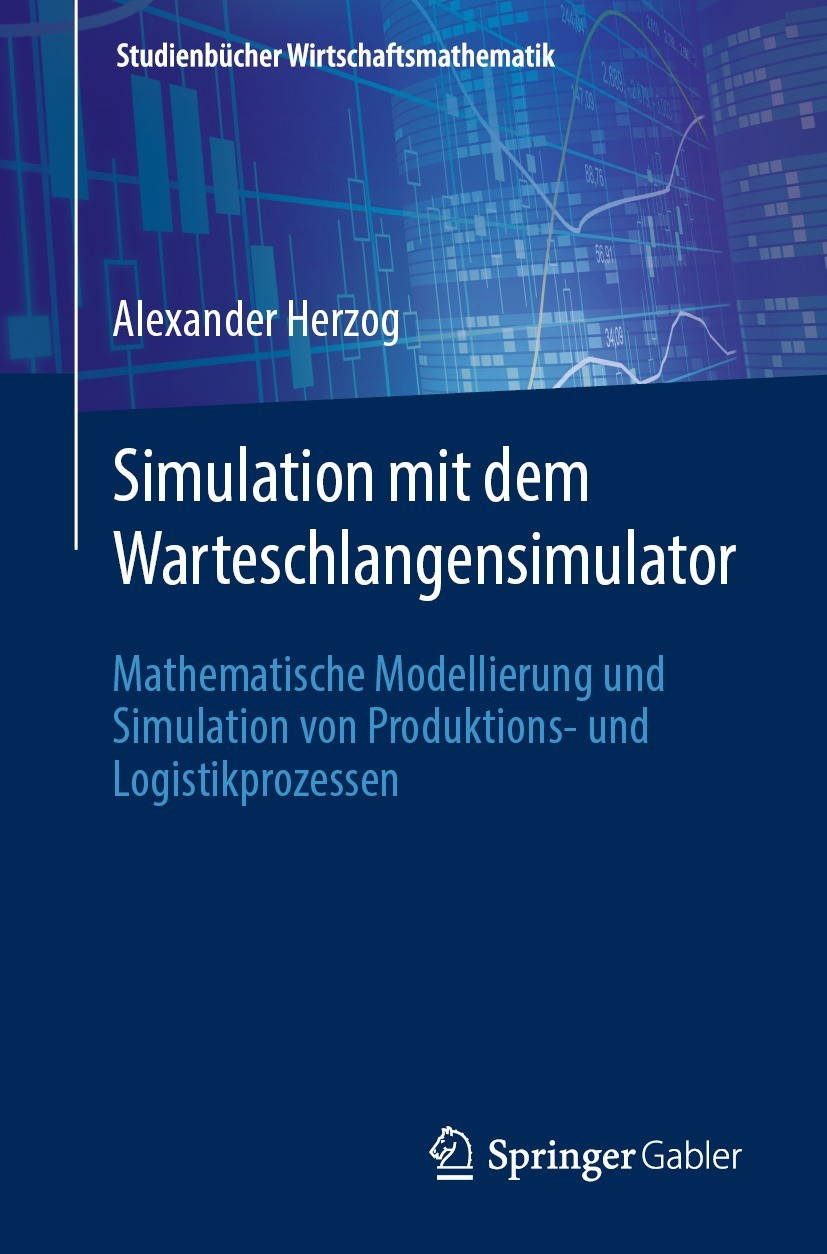
\includegraphics[width=6cm]{../BookCover.jpg}
\end{minipage}
\hfill
\begin{minipage}[b]{9.25cm}
Alexander Herzog:\\
\emph{Simulation mit dem Warteschlangensimulator},\\
Springer, 2021.
\vskip0.5em
ISBN: 978-3-658-34667-6
\vskip0.5em
\href{https://link.springer.com/book/10.1007/978-3-658-34668-3}{link.springer.com/book/10.1007/978-3-658-34668-3}
\end{minipage}

\end{document}